\documentclass[thesis.tex]{subfiles}

\begin{document}
\chapter{Survival analysis with perfect testing} \label{perf-test}

The estimation of incidence from prevalence is sensitive to the tail of the duration distribution.
In \cref{ATACCC} I estimated the duration distribution from the ATACCC data, however, this study suffered from a small sample size and only 20 days of follow-up.
\todo{Ref ATACCC chapter and in following paragraph}
Therefore, the estimation of the tail of the duration distribution is driven by model assumptions.
This chapter develops methods to estimate the distribution using CIS data, which has less frequent sampling but a large sample size and long follow-up.

I take a survival analysis approach to model the coarse sampling of the CIS (see \cref{perf-test:sec:problem}).
The problem of priors can be important to the results here, due to the lack of information in the data; in addition, the prior can be used to combine the information in the CIS with the results of \cref{ATACCC} (see \cref{perf-test:sec:parameters-priors}).
Through a simulation study (see \cref{perf-test:sec:simulation-study}), I show that these methods perform well, and in this context are not sensitive to model or prior specification.
However, application in reality must account for misclassification bias, the subject of \cref{imperf-test}.
\todo{Ref chapter incl misclassification}

\todo[inline]{%
  Somehwere, I need to fit in what exactly is novel here, and issues with the pre-existing work. What to cover is the application to both double interval censored and arbitrarily truncated data (which existed in some of the theoretical frameworks but not used); the issues with the conditional likelihood method of \textcite{bacchettiNonparametric}; and the lack of much work this century.
}

\section{Problem description and approach} \label{perf-test:sec:problem}

\todo[inline]{Some of these definitions likely need to be moved elsewhere as they will be needed in other chapters (e.g. ATACCC analysis).}
Consider the CIS data.
It consists of a series of tests on the same individuals (longitudinal data), where some individuals have a series of positive tests.
We wish to estimate the distribution of time for which an individual is positive for.
An individual could have multiple infections, and hence I refer to \emph{infection episodes}.

I define an individual as \emph{detectable} if they would test positive if tested, in the absence of misclassification error (which is dealt with in \cref{imperf-test}).
\todo{Ref chapter incl misclassification}
Episode $i$'s \emph{duration of positivity}, $D_i$ is the number of days that they are detectable for; I use time discretised to days, therefore, the duration is at least 1 day.
Note that the relationship between positivity (\ie the result of a PCR test) and infectiousness (\ie an individual's ability to pass on the virus) is complex, \todo{ref for PCR pos vs infectiousness} and beyond the scope of this thesis.
I define an episode as starting at time $B_i$ and ends at $E_i$, hence $D_i = E_i - B_i + 1$.

An episode is \emph{detected} when they test positive at least once, if this occurs; episode $i$ is detected at time $t$ if and only if: $i$ is detectable at $t$, $i$ is tested at $t$, and the test returns positive (a false negative does not occur).

Formally, the survival time function, parameterised by $\theta$, is the probability that an episode lasts at least $t$ days: $S_\theta(t) = \prob(D_i \geq t \mid B_i = b, \theta)$ where $D_i$ and $B_i$ are the duration and starting time of episode $i$ respectively.
We make the standard assumption that $D_i$ and $B_i$ are independent and hence: $S_\theta(t) = \prob(D_i \geq t \mid \theta)$.

I utilise survival analysis for analysing this data.
Survival analysis is the area of statistics concerned with estimating the distribution of the times between events.
It is broadly applicable to many domains, such as the time-to-failure for a mechanical system or the effect of a treatment on time spent in hospital.
In the context of this thesis, the distribution to estimate is that of duration of positivity.
The \emph{initiating event} is when the duration starts, \ie becoming detectable.
The \emph{terminating event} is when the duration starts, \ie becoming no longer detectable.

The reason for this approach, over modelling biomarkers (as in \cref{ATACCC}) is due to two factors.
\todo{Ref ATACCC chapter}
First, the large sample size in CIS means that approaches where the number of parameters scales with the number of observed infections (as it does with random effect based approaches) would be computationally challenging; this challenge is compounded by the data being stored in a trusted research environment limiting the computational power and tools available.
Second, the data is coarse with most episodes having only a single positive test; therefore, the trajectory of the viral load would not be well-identified in an individual.
Combined, these factors outweighed the downside of survival analysis only considering the binary outcome (\ie positive or negative) or the test rather than the additional information on the viral load.

The methods in this chapter deal with modelling two elements of the data-generating process, double interval censoring and truncation.
False negatives are not dealt with and left to \cref{imperf-test}.
\todo{Ref chapter incl misclassification}

Double interval censoring is a special case of censoring, a common and well-studied challenge encountered when dealing with survival data.
An event is \emph{censored} if the time of the event can only be bounded; it is \emph{left censored} if it is known to occur before a certain time, \emph{right censored} if it is known to occur after a certain time, and \emph{interval censored} if it is known to occur within an interval.
Interval censoring arises in CIS because we only observe the change from being not detectable (\ie: negative) at one test, to detectable (\ie: positive) at the following test and vice versa; \textcite{bogaertsSurvival} review many statistical methods applicable to interval censoring (see \cref{perf-test:fig:double-interval-censor}).
\emph{Double censoring} means that both the originating and terminating event are censored, and is also a well-studied problem, reviewed by \textcite{sunStatisticala}.
In CIS, we have \emph{double interval censoring} meaning that both the initiating and the terminating events are interval censored.
\begin{figure}
  \centering 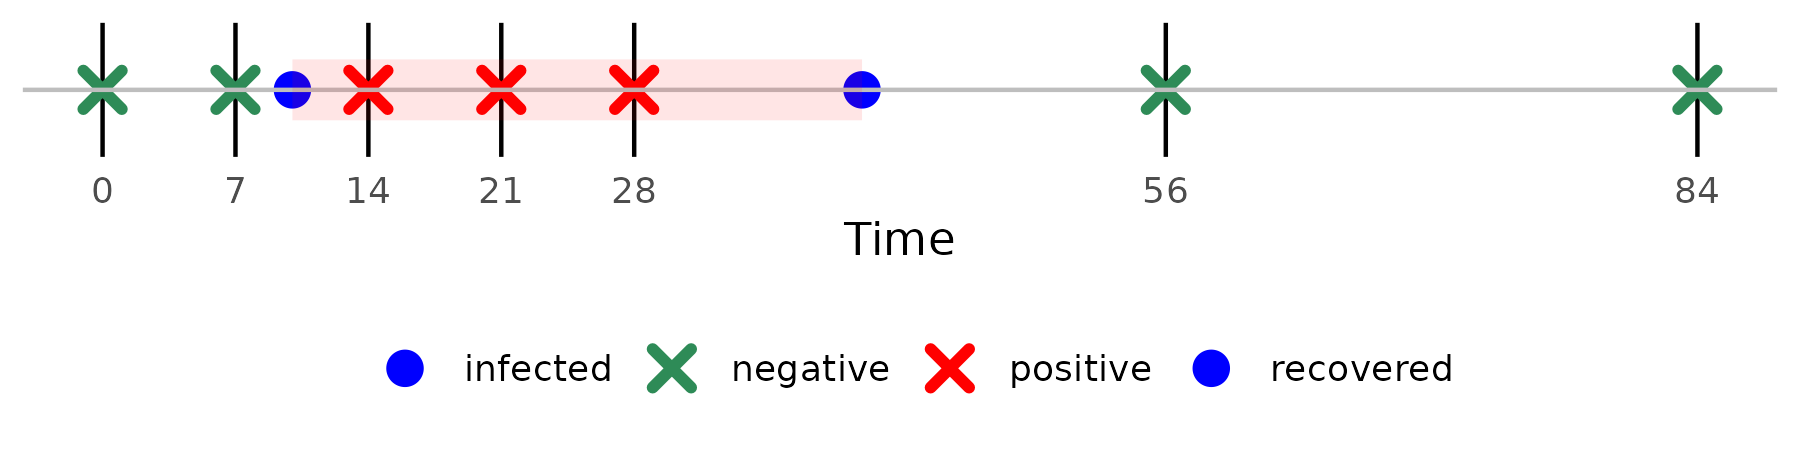
\includegraphics{cis-perfect-testing/double-interval-censor}
  \caption{Episodes data in CIS is double interval censored, meaning that both the start and end of the episode are only known up to an interval. Demonstrated here by a participant who transitions negative at time 7 to positive at time 14, bounding the start of the episode; similarly, the transition positive at time 28 to negative at time 56 bounds the end of the episode. \label{perf-test:fig:double-interval-censor}}
\end{figure}

Interval censoring is a well-studied area in the biostatistics and broader statistical literature\todo{interval censoring refs}.
Double interval censoring is less frequent, although has been considered previously\todo{double interval censoring refs}.

The second element is truncation.
Truncation occurs because we do not observe some episodes: an episode can occur between tests and hence the episode is never detected (see \cref{perf-test:fig:truncation}).
We do not know how many infections we do not detect.
Failure to model truncation will lead to estimating too long durations because the detected episodes are a biased sample with a longer duration.
To see why they are shorter, consider the undetected infection in the bottom of \cref{perf-test:fig:truncation}.
This individual was infected at time 33 for 10 days.
If instead there infection was 24 days (or longer), the individual would still have been detectable at their next test, and therefore would have been detected.

Truncation is a large problem when individuals move to the infrequent testing schedule within CIS.
Consider that, based on the estimates in \cref{ATACCC}, the median length of an episode is 14 days \todo{check this number} we would not expect many episodes to last the 28 days that can occur between tests.
\todo{Ref ATACCC chapter}
\begin{figure}
  \centering 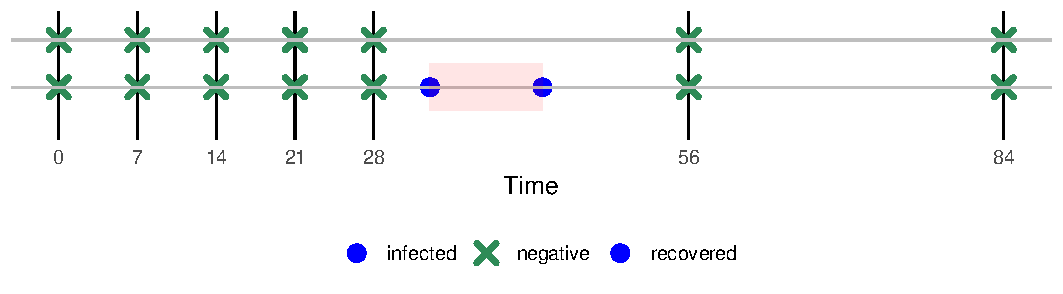
\includegraphics{cis-perfect-testing/truncation}
  \caption{Episodes data in CIS is truncated, meaning that an unknown number of infections are never detected. Consider the two individuals shown here: we collect identical data for them (a series of negative tests) yet the top individual was never infected and the bottom individual was. See the main text for why this is an issue. \label{perf-test:fig:truncation}}
\end{figure}

This combination of censoring and truncation are rarely encountered in biomedical data\todo{refs to combining double interval censoring with truncation}.

While this chapter sets up the framework for analysing the CIS data, applying the method to CIS data requires modelling false negatives.
That is the subject of \cref{imperf-test} and hence a full description of the data and processing of it is deferred to that chapter.
\todo{Ref chapter incl misclassification}

\section{Modelling the duration}\label{perf-test:sec:model}
Now I develop a model accounting for double interval censoring and truncation, building on prior work in both biomedical and bird nesting studies.
The arbitrary nature of truncation in CIS, where each individual has a unique truncation pattern and is neither simple left nor right truncation, has not previously been explored in the literature.
Furthermore, I explore a Bayesian framework where the amount of explicit data augmentation is limited allowing the method to scale to the large number of episodes present in CIS without requiring vast computing resources (such as a high-performance cluster).
Only limited resources are available within the secure research service (SRS, a form of trusted research environment) where the CIS data is held.
Therefore, unlike most Bayesian methods (e.g.: \textcite{heBayesiana}, \textcite{heBayesian}, and \textcite{caoModeling}) we avoid augmenting the data with unobserved times of infection or any information on the truncated infections; this is due to the large number of infections (>4000 in the time period considered) making this approach computationally expensive.

I model only individuals with detected episodes.
This approach is based on long-standing methodology~\autocites{heiseyModelling}{dempsterMaximum}{turnbullEmpirical}.
The conceptual approach here is to form a cohort of individuals for which we observe at least one positive test, and then consider a study which had only enrolled these individuals.
The modelling approach then corrects for this selection bias, by considering \emph{ghost} infections that occur in identical individuals but were truncated.

I have also considered a model including individuals without any observed episodes (see \cref{appendix:total-model} for details).
These individuals may have truncated episodes or may not have been infected at all.
However, I found that this model has little difference in results while increasing computational complexity and requiring assumptions on reinfection (discussed in \cref{perf-test:sec:discussion}).

\subsection{Notation and assumptions}
\todo[inline]{Some of this will possibly be defined elsewhere, such as in the introduction where CIS is introduced}
\begin{itemize}
\item
  Time is discrete: $1, \dots, T$.
\item
  We observe $n_a$ episodes of infection, indexed by $i$.
\item
  The $i$ in which episode $i$ occurs is tested at times
  $t_i = \{ t_{i,1}, \dots, t_{i,m_i} \}$.
\item
  Each observed episode has an unknown start of infection time $b_i$
  and end of infection time $e_i$ (the first and last day that the
  individual would test positive due to this episode respectively).
  These are realisations of the random variables $B_i$ and $E_i$
  respectively.
\item
  The duration of the infection is the number of days for which an
  individual tests positive, $D_i = E_i - B_i + 1$.
\item
  We assume that, for all episodes $i$, $D_i$ is iid and independent
  of the time of the infection. Define the survival function
  $\prob(D_i \geq t \mid B_i = b, \theta) = \prob(D_i \geq t \mid \theta) = S_\theta(t)$,
  where $\theta$ are the parameters controlling the survival
  distribution (the discussion in this document is valid regardless of
  the model specified for $S_\theta$ and hence we consider $\theta$
  as an arbitrary vector of parameters).
\item
  The beginning of episode $i$ is known to occur in the interval
  $[l_i^{(b)}, r_i^{(b)}]$, and similarly for the end of the infection
  in $[l_i^{(e)}, r_i^{(e)}]$.
\item
  $y_i(t)$ for $t \in t_i$ is a binary indicator giving the test
  result for individual $i$ at time $t$. Under the perfect testing
  assumption, $y_i(t) = 1$ if and only if $b_i \leq t \leq e_i$.
\item
  Throughout, the convention that lower-case letters are realisations of
  upper-case random variables is used.
\end{itemize}

\subsection{Likelihood}\label{perf-test:sec:likelihood}

Episode $i$ can be fully characterised by the pair $(b_i, e_i)$ of
start and end dates of the episode, which belong to the state space
$T \times T$. If the individual in which the episode occurs is tested
between $b_i$ and $e_i$ (inclusive), then we observe the episode,
otherwise it is truncated. For the $i$th episode that we observed, we
consider there is an unknown number, $n_{it}$, where $(b, e)$ are
drawn from the same distribution as those that lead to episode $i$,
and occur in an (imagined) individual identical to $i$, but were
truncated. Episodes are also truncated if there is no negative test
prior to their start, that is, the individual the episode occurred in
had no tests before $b_i$. The truncated episodes are the ghosts of $i$.

\Textcite{heiseyModelling} provide a framework for formalising this.
Define three sets which partition the space of possible infection and
recovery (\ie: are strict subsets of $T \times T$) given the
observations associated with episode $i$ (graphically shown in Figure
\ref{perf-test:fig:partitionSpace}). Each episode, whether observed or not, must
fall into one of these three classes with a probability that is a
function of $\theta$ (see section \ref{perf-test:sec:likelihood}).

\begin{itemize}
\item
  Admissible episodes, $\alpha_i$, which have an infection and
  recovery time within their respective intervals observed.
  $n_{ia} =1$ of these occurred, each with probability
  $p_{ia} = \prob((b, e) \in \alpha_i \mid \theta)$.
\item
  Truncated episodes, $\Omega_i^C$, which have an infection and
  recovery time such that they would not have tested positive. An
  unknown number, $n_{it}$ of these observed, each with probability
  $p_{it} = \prob((b, e) \in \Omega^C_i \mid \theta)$.
\item
  Inadmissible episodes, $\beta_i$, which do not have an infection and
  recovery time within their respective intervals but would have been
  observed (not truncated). This is all remaining episodes not in the
  previous sets. $n_{iu} = 0$ of these occurred, where they would have
  occurred with probability
  $p_{iu} = \prob((b, e) \in \beta_i \mid \theta)$.
\end{itemize}

The untruncated region (where we could have observed an episode) is
$\Omega_i = \alpha_i \cup \beta_i$ (the notation here is used for
consistency with \textcite{heiseyModelling}), and is the
complement of $\Omega^C_i$.

\begin{figure}
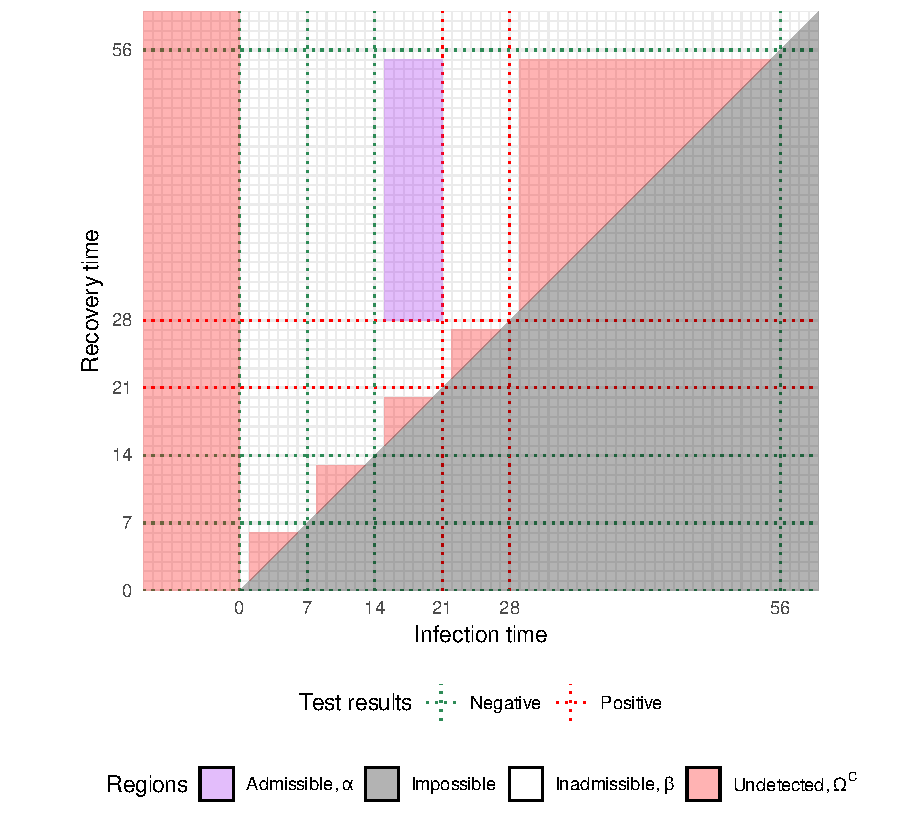
\includegraphics[width=\textwidth]{cis-perfect-testing/regions_diag}
\caption{Admissible, $\alpha_i$, inadmissible, $\beta_i$ and
untruncated, $\Omega_i^C$ regions for an episode $i$ in an
individual whose first test was at time 0 and negative, with subsequent
negative tests at times 7, 14, and 56, and positive tests at times 21
and 28. \label{perf-test:fig:partitionSpace}}
\end{figure}

These three classes span all possible episodes and are mutually
exclusive, and hence the total number of episodes,
$n_i = n_{ia} + n_{iu} + n_{it}$, and
$p_{ia} + p_{iu} + p_{it} = 1$.

Episode $i$ and its ghosts independently occur belong to one of these
classes. Therefore, conditional on $n_i$, the number of episodes in
each class (that is, the counts $n_{ia}, n_{iu}, n_{it}$) are
distributed multinomially. Hence:
\begin{align}
&p(n_{ia} = 1, n_{iu} = 0, n_{it} = n_i - 1 \mid n_i, \theta) \\
&= \frac{n_i!}{n_{ia}! n_{iu}! (n_i- n_{ia} - n_{it})!} p_{ia}^{n_{ia}} p_{ua}^{n_{ia}} p_{it}^{n_i- n_{ia} - n_{it}} \\
&= \frac{n_i!}{(n_i-1)!} p_{ia} p_{it}^{n_i- 1} &\text{as $n_{ia} = 1$ and $n_{iu} = 0$}\\
&= n_i p_{ia} p_{it}^{n_i- 1}
\end{align}

The posterior we are interested in is
$p(\theta \mid n_{ia} = 1, n_{iu} = 0, \dots, n_{n_a,a} = 1, n_{n_a,u} = 0)$,
where $\theta$ are the parameters governing the survival distribution
and hence allow derivation of the $p$s.
\begin{align}
&p(\theta \mid n_{ia} = 1, n_{iu} = 0, \dots, n_{n_a,a} = 1, n_{n_a,u} = 0) \\
&\propto p(\theta) \prod_{i=1}^{n_a} p(n_{ia} = 1, n_{iu} = 0 \mid \theta) \\
&= p(\theta) \prod_{i=1}^{n_a} \sum_{n_i=1}^\infty p(n_{ia} = 1, n_{iu} = 0, n_{it} = n_i - 1 \mid \theta, n_i) p(n_i \mid \theta) \\
&= p(\theta) \prod_{i=1}^{n_a} \sum_{n_i=1}^\infty n_i p_{ia} p_{it}^{n_i- 1} p(n_i) \\
&= p(\theta) \prod_{i=1}^{n_a} p_{ia} \sum_{n_i=1}^\infty n_i p_{it}^{n_i- 1} p(n_i)
\end{align}
where the last line follows by assuming prior independence.

In the remainder of the section, we derive the expressions for $p_{ia}$ and
$p_{it}$ in terms of the data, and analytical solutions for the sum
under different priors.

I derive an analytical solution to $\sum_{n_i=1}^\infty n_i p_{it}^{n_i- 1} p(n_i)$ under two different assumptions for $p(n_i)$.
First, we consider the improper prior $p(n_i) \propto 1/n_i$, this prior has several attractive properties.
Then, we consider a negative binomial distribution (which includes the geometric and Poisson distributions as a special and limiting case respectively).

The prior $p(n_i) \propto 1/n_i$ means that the model coincides with the frequentist conditional likelihood approach, up to the priors on other parameters~\cites[section 4.2]{dempsterMaximum}{heiseyModelling}[section 8.7.5]{gelmanBayesian}.
Furthermore, this is the reference prior for this quantity\autocite{heBayesiana}.
Under this prior,
$\sum_{n_i=1}^\infty n_i p_{it}^{n_i- 1} p(n_i) \propto \sum_{n_i=1}^\infty p_{it}^{n_i-1} = 1/(1-p_{it})$.
% (\protect\hyperlink{ref-dempsterMaximum}{Dempster, Laird, and
% Rubin} (\protect\hyperlink{ref-dempsterMaximum}{1977}) section 4.2;
% \protect\hyperlink{ref-heiseyModelling}{Heisey and Nordheim}
% (\protect\hyperlink{ref-heiseyModelling}{1995});
% \protect\hyperlink{ref-gelmanBayesian}{Gelman et al.}
% (\protect\hyperlink{ref-gelmanBayesian}{2013}) section 8.7.5)

Now consider $N_i \dist \NegBin(\mu, r)$ using the
mean/dispersion parameterisation of the negative binomial. Equivalently:
\begin{align}
N_i \mid \lambda &\dist \Poi(\lambda) \\
\lambda &\dist \GamDist(a, b)
\end{align}
where $b = r / \mu$ and $a = r$.
Hence:
\begin{align}
\sum_{n_i=1}^\infty n_i p_{it}^{n_i- 1} p(n_i) 
&= \int \sum_{n_i=1}^\infty n_i p_{it}^{n_i- 1} p(n_i \mid \lambda) p(\lambda) d\lambda \\
&= \int \sum_{n_i=1}^\infty n_i p_{it}^{n_i- 1} \frac{\lambda^{n_i} e^{-\lambda}}{n_i!} p(\lambda) d\lambda \\
&= \int e^{-\lambda} \sum_{n_i=1}^\infty p_{it}^{n_i- 1} \frac{\lambda^{n_i-1}\lambda }{(n_i-1)!} p(\lambda) d\lambda \\
&= \int e^{-\lambda} \lambda p(\lambda) \sum_{n_t=0}^\infty p_{it}^{n_t} \frac{\lambda^{n_t} }{n_t!} d\lambda &n_t = n_i - 1 \\
&= \int e^{-\lambda} \lambda p(\lambda) e^{p_{it}\lambda} d\lambda &\text{Poisson pmf} \\
&= \int e^{\lambda (p_{it} - 1)} \lambda p(\lambda) d\lambda \\
&= \int e^{\lambda (p_{it} - 1)} \frac{b^a}{\Gamma(a)} \lambda^{a-1} e^{-b\lambda} \lambda d\lambda \\
&= \frac{\Gamma(a+1)b^a}{\Gamma(a) (b+1-p_{it})^{a+1}} \\ 
  &\; \times \int \frac{(b+1-p_{it})^{a+1}}{\Gamma(a+1)} \\
  &\; \lambda^{(a+1)-1} e^{-(b+1-p_{it})\lambda} d\lambda \\
&= \frac{\Gamma(a+1)b^a}{\Gamma(a) (b+1-p_{it})^{a+1}} &\text{as gamma pdf} \\
&\propto (b+1-p_{it})^{-(a+1)} \\
&= (r/\mu+1-p_{it})^{-(r+1)} \\
&\propto (r+\mu (1-p_{it}))^{-(r+1)}
\end{align}
Note that $r=0$ recovers the previous derivation (up to
proportionality).

The above allows us to sample from the posterior without needing to
sample the $n_i$s. This is convenient because there are as many
$n_i$s as episodes observed and hence is computationally costly to
sample. Furthermore, each $n_i$ is a discrete parameter, and hence
cannot be sampled within the current Stan implementation.

Having estimated the posterior of the other parameters, we might want to
consider the posterior of $n_i$ (normally for diagnostic or model
debugging purposes), which we can sample from the full conditional.
Specifically, for each posterior sample of $\theta$, we sample one
draw from $n_i \mid \theta, y$ where $y$ represents all the data.

Due to the conditional independence of the $n_i$s, we find that:
\begin{align}
&p(n_i \mid \theta, n_{ia} = 1, n_{iu} = 0) \\
&\propto p(n_{ia} = 1, n_{iu} = 0, n_{it} = n_i - 1 \mid n_i, p_{iu}, p_{ia}, p_{it}) p(n_i) \\
&\propto n_i p_{it}^{n_i- 1} p(n_i)
\end{align}
With the prior, $p(n_i) \propto 1/n_i$ then this is a geometric
distribution with parameter $1 - p_{it}$. With a negative binomial
prior, we have:
\begin{align}
n_i p_{it}^{n_i- 1} p(n_i)
&\propto n_i p_{it}^{n_i- 1} \frac{\Gamma(r + n_i)}{n_i!} \left( \frac{\mu}{r+\mu} \right)^{n_i} \\
&\propto \frac{\Gamma((r + 1) + (n_i - 1))}{(n_i-1)!} \left( \frac{\mu p_{it}}{r+\mu} \right)^{n_i-1}
\end{align}
which is a negative binomial pmf with size parameter $r+1$ and
probability parameter $\frac{r + \mu (1 - p_{it})}{r+\mu}$. The mean
of this is
\begin{align}
\frac{(r+1)\mu p_{it}}{r+\mu(1-p_{it})}
\end{align}

Next, I derive $p_{ia}$ and $p_{it}$.

By definition, we have
\begin{align}
p_{ia} &= \prob((b, e) \in \alpha_i) \\
\alpha_i &= \{ (b, e) : l_i^{(b)} \leq b \leq r_i^{(b)} \wedge l_i^{(e)} \leq e \leq r_i^{(e)}\}.
\intertext{Hence:}
p_{ia}
&= \prob \left( l_i^{(b)} \leq B_i \leq r_i^{(b)}, l_i^{(e)} \leq E_i \leq r_i^{(e)} \right) \\
&= \prob \left( l_i^{(e)} \leq E_i \leq r_i^{(e)} \mid l_i^{(b)} \leq B_i \leq r_i^{(b)} \right) \prob \left( l_i^{(b)} \leq B_i \leq r_i^{(b)} \right) \\
&=\sum_{b = l_i^{(l)}}^{r_i^{(b)}} \prob \left( l_i^{(e)} \leq E_i \leq r_i^{(e)} \mid B_i = b \right) \prob \left(B_i = b \right) \\
&=\sum_{b = l_i^{(b)}}^{r_i^{(b)}} \prob \left( l_i^{(e)} - b + 1 \leq D_i \leq r_i^{(e)} - b + 1 \right) \prob \left(B_i = b \right) \\
&=\sum_{b = l_i^{(b)}}^{r_i^{(b)}} \left( S_\theta(l_i^{(e)} - b + 1) - S_\theta(r_i^{(e)} - b + 2) \right) \prob \left(B_i = b \right) \\
&\propto \sum_{b = l_i^{(b)}}^{r_i^{(b)}} \left( S_\theta(l_i^{(e)} - b + 1) - S_\theta(r_i^{(e)} - b + 2) \right)
\end{align}
under the assumption of uniform probability of infection time.

Next, we derive $p_{it} = \prob((b, e) \in \Omega^C_i)$, the probability
that episode $i$ was truncated. A truncated episode means that no test
was performed during the episode or there was no negative test prior to
the episode. Denote by $t_i$ the set of testing times for the
individual in which episode $i$ was observed, and define the time
until the next test on the individual after time $t'$ as:
\begin{align}
t^N_{it} &= \min \{ t' \in t_i : t' \geq t \} - t.
\intertext{Then:}
\Omega^C_i
&= \{ (b, e) : \nexists t \in t_i. b \leq t \leq e \vee b \leq \min(t_i) \} \\
&= \{ (b, e) : e - b < t^N_{ib} \vee b \leq \min(t_i) \}.
\intertext{Hence:}
1 - p_{it}
&= 1 - \prob(E_i - B_i < t_{iB_i}^N \vee B_i \leq \min(t_i)) \\
&= 1 - \prob(E_i - B_i < t_{iB_i}^N \wedge B_i > \min(t_i)) - \prob(B_i \leq \min(t_i)) \\
&= 1 - \sum_{b=\min(t_i) + 1}^T \prob(E_i - b + 1 < t_{ib}^N \mid B_i = b) \prob(B_i = b) \\
  &\; - \sum_{t=1}^{\min(t_i)} \prob(B_i = b)\\
&= 1 - \frac{1}{T} \sum_{b=\min(t_i)+1}^T (1 - S_\theta(t_{ib}^N + 1)) - \frac{\min(t_i)}{T} \\
&= 1 - \frac{T-\min(t_i)}{T} + \frac{1}{T} \sum_{b=\min(t_i)+1}^T S_\theta(t_{ib}^N + 1)) - \frac{\min(t_i)}{T} \\
&= \frac{1}{T} \sum_{b=\min(t_i)+1}^T S_\theta(t_{ib}^N + 1)
\end{align}

\subsection{Full posterior}\label{perf-test:sec:full-posterior}

Under the prior $p(n_i) \propto 1/n_i$:
\begin{align}
&p(\theta \mid n_{ia} = 1, n_{iu} = 0, \dots, n_{n_a,a} = 1, n_{n_a,u} = 0) \\
&\propto p(\theta) \prod_{i=1}^{n_a} p_{ia} \sum_{n_i=1}^\infty n_i p_{it}^{n_i- 1} p(n_i) \\
&= p(\theta) \prod_{i=1}^{n_a} \frac{p_{ia}}{1-p_{it}} \\
&\propto p(\theta) \prod_{i=1}^{n_a} \frac{\sum_{b = l_i^{(b)}}^{r_i^{(b)}} \left( S_\theta(r_i^{(e)} - b - 1) - S_\theta(l_i^{(e)} - b - 1) \right)}{\sum_{b=\min(t_i)}^T S_\theta(t_{ib}^N + 1)} \\
\end{align}

Under the prior $N_i \dist \text{NegBinom}(\mu, r)$:
\begin{align}
&p(\theta \mid n_{ia} = 1, n_{iu} = 0, \dots, n_{n_a,a} = 1, n_{n_a,u} = 0) \\
&\propto p(\theta) \prod_{i=1}^{n_a} p_{ia} \sum_{n_i=1}^\infty n_i p_{it}^{n_i- 1} p(n_i) \\
&= p(\theta) \prod_{i=1}^{n_a} \frac{p_{ia}}{(r+\mu (1-p_{it}))^{(r+1)}} \\
&= p(\theta) \prod_{i=1}^{n_a} \frac{\sum_{b=l_i^{(b)}}^{r_i^{(b)}} \left( S_\theta(r_i^{(e)} - b - 1) - S_\theta(l_i^{(e)} - b - 1) \right)}{\left( r+\mu/T \left( \sum_{b=\min(t_i)}^T S_\theta(t_{ib}^N + 1) \right) \right)^{(r+1)}} \\
\end{align}

\section{Parameterisation and priors for the survival function} \label{perf-test:sec:parameters-priors}

The form of $S_\theta(t)$ is yet to be specified.
As frequently observed in the literature\todo{refs for parameterisation}, it is more convenient to operate with the hazard than the survival or probability mass function directly.
This is because the mass function must sum to one and the survival must be monotonically decreasing, while there are no constraints across multiple hazards.
The only constraint on the hazard is to be in the interval $[0, 1]$, since they are probabilities.

In this section, I consider the various parameterisation of the survival function that are available.
This has implications for the choice of prior it is not possible to be vague on all sensible parameterisations.
Informative priors might also be attractive, and allow the incorporation of the estimates from \cref{ATACCC}.
\todo{Ref ATACCC chapter}

The hazard is convenient to use because it is unconstrained except in the interval [0, 1]\todo{ref where been used previously}.
Survival needs to be monotonic.

\subsection{Independent priors}

A common assumption throughout Bayesian analyses is independence of the parameters in the prior.
This is convenient because we can then use univariate distributions.
\todo{This feels a bit clumsy/patronising to the reader. Maybe change the phrasing?}
A Beta distribution for each hazard parameter, $\lambda_t$, is a natural choice due to it being a probability.

An uninformative prior would be $\lambda_t \dist \Beta(\alpha, \alpha)$, with common choices of $\alpha$ being $0.5$, Jeffreys' Prior, or $1$, a flat prior.
Flat or uninformative priors on the hazard lead to very informative priors on the survival, favouring short survival times.
The sharp falloff can be seen by noting that these priors have expectation 0.5, hence $\E(S(t)) = \E \left( \prod_{i=1}^{t-1} (1-\lambda_t) \right) = 0.5^{t-1}$ which decreases very quickly.
Our prior belief is not well-represented by this prior, and in fact a priori viewed as extremely unlikely (see \cref{perf-test:fig:flat-priors}),
Therefore, I favour a prior which is weakly informative on the survival, or an informative prior used to represent our belief from the \cref{ATACCC} analysis.
\todo{Ref ATACCC chapter}
\begin{figure}
  \centering 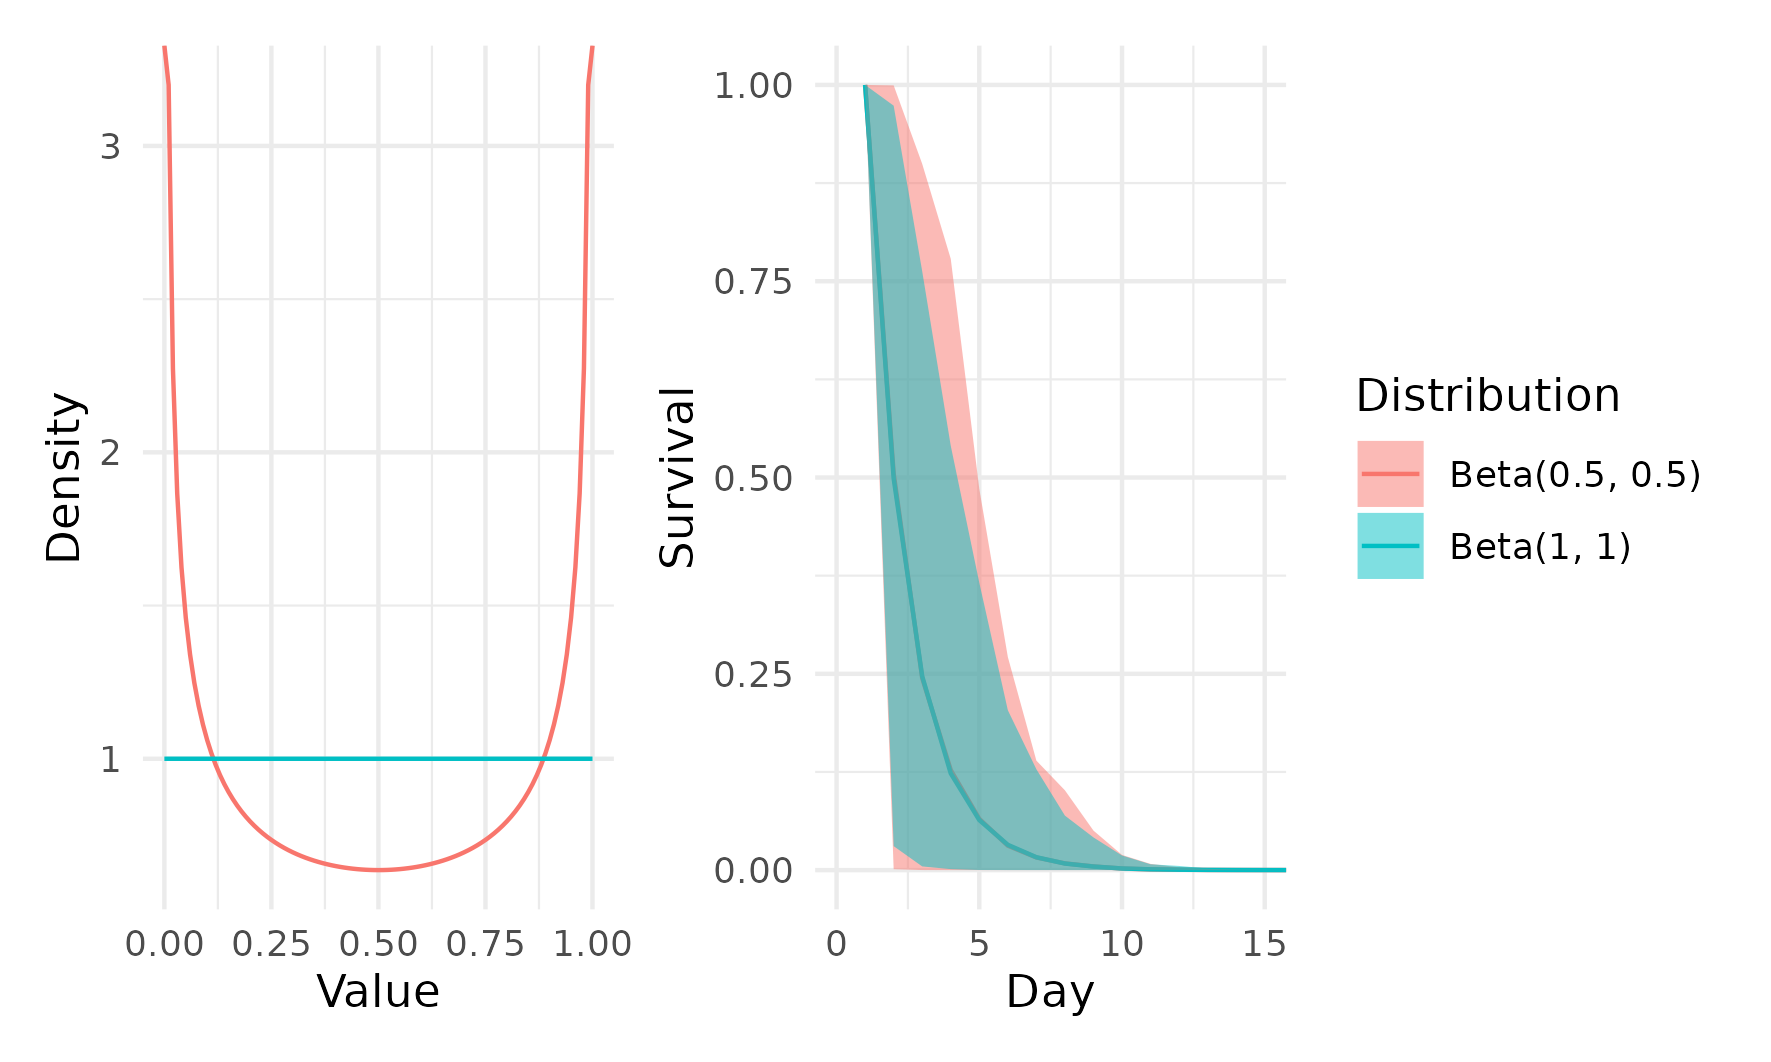
\includegraphics{cis-perfect-testing/flat-prior}
  \todo[inline]{Create flat priors figure}
  \caption{The prior predictive survival time (shown) is very short when using either a Beta(1, 1) flat prior or Beta(0.5, 0.5) uninformative prior on the hazard at each time. \label{perf-test:fig:flat-prior}}
\end{figure}

Instead, I propose a weakly informative prior Beta(0.1, 1.9), linking to previous literature for a point estimate and showing vague figures.

A Beta(0.1, 1.9) prior has mean 0.05 while not having much information (the informativeness of a Beta distribution is related to $\alpha + \beta$ which here equals 2, the same as the flat prior case); and the central 95\% mass is 0.00-0.47.
The central estimate reflects previous estimates that the median duration is in the range 15-20 days~\autocite{cevikShedding}, which would translate to hazard of around 0.05.
The prior predictive distribution on the survival time implied by this prior is very vague (see \cref{perf-test:fig:vague-prior}).
\begin{figure}
  \centering %\includegraphics{cis-perfect-testing/vague-priors}
  \todo[inline]{Create vague prior figure}
  \caption{The prior predictive survival time (shown) is very vague using a Beta(0.1, 1.9) prior. \label{perf-test:fig:vague-prior}}
\end{figure}

\subsection{Informative priors}

The analysis in \cref{ATACCC} can be used to provide prior information for the CIS analysis.
\todo{Ref ATACCC chapter here and next few}
In particular, the ATACCC study frequently samples individuals early in the infection.
Therefore, the survival distribution from that analysis should be reliable through this period.
CIS can then inform the remainder of the distribution where the previous analysis is based on extrapolation.

The model structure assumed in \cref{ATACCC} leads to positive correlation in the posterior estimates of the hazard.
\todo{Ref ATACCC chapter}
It is important to propagate this correlation as part of the prior uncertainty into the present analysis.
We do this in two parts: first, approximate the previous posterior estimate of the logit-hazard as a multivariate normal (which can be viewed as an approximation of Markov melding~\autoref{goudieJoining}).
Then, use a Beta process to add additional uncertainty to this.

There are two reasons to increase the uncertainty relative to the \cref{ATACCC} posterior.
First, we do not have full belief in these estimates due to the extrapolation problem previously discussed.
Second, the results may not fully generalise between the two studies.
The samples are tested using different laboratories, with different PCR machines, and hence may not have the same characteristics~\autocite{punchooLaboratory}.
The study participants, while both targeting a general population cohort, may also differ because ATACCC recruited through NHS Test and Trace while CIS recruited by sampling from a database of addresses (see \cref{intro:sec:data}).

The first step, approximating the \cref{ATACCC} posterior as a multivariate normal, is done through the method of moments.
The approximation is very good (see \cref{perf-test:fig:approximate-ATACCC}).

The discrete Beta process prior generalises the form of prior used in the previous section, allowing the central estimate of the hazard to vary over time~\autocites{ibrahimBayesian}{sunStatisticala}.
\begin{align}
  \lambda_t &\sim \text{Beta}(\alpha_t, \beta_t) &t = 1, 2, \dots \\
  \alpha_t &= c_t h_t + \alpha_0 \\
  \beta_t &= c_t (1 - h_t) + \beta_0
\end{align}
where $k_t$, $\alpha_0$, and $\beta_0$ are hyperparameters; and $h_t$ is a point estimate of the hazard at time $t$ from ATACCC.
An intuition for what this distribution represents can be gained by considering the conjugate model for $\lambda_t$ with a beta prior and a binomial likelihood.
If $\lambda_t$ is given the prior distribution $\text{Beta}(\alpha_0, \beta_0)$, and we then have $k_t$ observations with $k_t h_t$ successes, then the posterior distribution for $\lambda_t$ is $\text{Beta}(\alpha_t, \beta_t)$ (as defined above).


\subsection{Smoothing priors}

A final possible prior are ones to favour smoothness in the hazard.
This is the Bayesian equivalent of a penalised likelihood, used frequently in the non-parametric frequentist setting.
Biological and epidemiological considerations mean that it would be surprising if the hazard varied significantly day-to-day.
A smoothing prior encodes this information within the analysis.

I consider two forms of smoothing priors: first-order and second-order random walks on the logit-hazard, $\logit(\lambda_t) = \log(\lambda_t) - \log(1 - \lambda_t)$.
The logit transformation maps from the $[0, 1]$ interval to the full real line.
\todo{The logit intro will be in the previous subsection}
Random walks are a very common form of smoothing prior for discrete time.

A first-order random walk prior encodes that the hazard should be constant with some random changes at each time step.
\begin{align}
  \logit\lambda_{t+1} &= \logit\lambda_t + \sigma \epsilon_t &\text{for $t \geq 1$} \\
  \epsilon_t &\dist N(0, 1) \\
  \logit \lambda_1 &\dist N(\mu_1, \sigma_1^2)
\end{align}
The hyperparameter $\sigma$ controls the standard deviation of the random walk, and the prior on $\lambda_1$ gives the starting point of the random walk.
Smaller values favour a smoothing process.

A second-order random walk prior encodes that the hazard should be linearly changing with some random changes at each time step.
\begin{align}
  \logit\lambda_{t+1}
  &= \logit\lambda_t + (\logit\lambda_t - \logit\lambda_{t-1}) + \sigma \epsilon_t &\text{for $t \geq 2$} \\
  &= 2\logit\lambda_t - \logit\lambda_{t-1} + \sigma \epsilon_t \\
  \epsilon_t &\dist N(0, 1) &\text{for $t \geq 2$}  \\
  \logit\lambda_2 &= \logit\lambda_1 + \epsilon_1 \\\
  \epsilon_1 &\dist N(\mu_2, \sigma_2^2) \\
  \logit \lambda_1 &\dist N(\mu_1, \sigma_1^2)
\end{align}
The hyperparameter $\sigma$ controls the standard deviation of the random walk, and there is an additional prior on $\epsilon_1$ for the initial gradient of the change in the hazard.

\section{Simulation study} \label{perf-test:sec:simulation-study}

\subsection{Setup}

I simulate each individual enrolled in CIS who was tested at least once between ?? and ??.
All their tests between ?? and ?? are considered, and each individual is assigned an infection time $B_i$ uniformly at random from ??.
\todo{check dates and periods}

I take as the ground truth distribution for duration of positivity a combination of the estimates from \cref{ATACCC} with an inflated tail to represent what is seen within CIS.
\todo{Ref ATACCC chapter}
The tail is modified based on Sarah Walker's (unpublished) work based on CIS data.
These curves and the combined curve are compared in \cref{perf-test:fig:duration-dist}.
Individual $i$'s duration of positivity, $D_i$, is then an independent draw from this distribution.

\begin{figure}
  \todo[inline]{Find figure comparing different duration distributions}
  \caption{Comparison of the duration distributions, see main text for details of how each is derived. \label{perf-test:fig:duration-dist}}
\end{figure}

Sarah uses survival analysis to estimate the duration from CIS data.
The initiating event is assumed known as the time the episode was detected.
The final event is assumed interval-censored between the time of the final positive test and the subsequent negative test, or right-censored if a negative test has not yet been observed.
A flexible, spline-based form is assumed for the baseline survival function~\autocite{roystonSTPM,roystonFlexible} with covariates introduced via proportional odds.
By not accounting for either the truncation or the interval censoring of the initiating event, this analysis has competing biases which makes them hard to interpret~\autocite{cisMethodsONS}.

% \todo[inline]{The following seems important to justify why we can't just use these estimates but is also basically an aside}
% We know of two biases introduced from this analysis.
% \enquote{There is a bias in estimating the clearance distribution because the analysis used to estimate how long a person stays positive only starts from their first positive test.
% Since (most) people will have become positive on an earlier day, this will bias the clearance curves downwards (making the estimates too short).
% However, there is another bias due to the survey missing positive episodes entirely if they are short.
% This means that our dataset has fewer short positive episodes than in the population as a whole, and that the sample used to run the survival analysis is biased towards people with longer positive episodes.
% This will bias the clearance curves upwards (making the estimates too long).}~\autocite{cisMethodsONS}.

To form the duration distribution used in the simulation, we combine these two estimates.
The first 30 days of the distribution is proportional to the ATACCC estimate, with the rest proportional to this CIS-based estimates.
% The CIS-based estimates are shifted 3 days in order to make this smooth; this counteracts the above bias of missing the start of the infection (for times above 30 days, the other bias, missing short infections, is negligible). ERR... I'M NOT DOING THIS ANYMORE OH NO!!
Denote by $f_A(t)$ the distribution function estimated from ATACCC and $f_C(t)$ that from these CIS-based estimates.
Define:
$$
f_S'(t) = \begin{cases}
	f_A(t) &t \leq 30 \\
	f_C(t) &t > 30
\end{cases}
$$
Then the distribution used in the simulation is the normalised version of this: $f_S(t) = f'_S(t)/\sum_i f_S'(i)$.

The first day individual $i$ can be positive is their day of infection, $B_i$, the last day is $E_i = B_i + D_i - 1$ where $D_i$ is the duration of positivity for individual $i$, drawn from $f_S$.
Any test between $B_i$ and $E_i$ (inclusive) is positive; outside this period, all tests are negative.

I then filter the episodes to replicate the process which will be used when working with the CIS data.
First, discard any episodes where there are no positive tests as they are never detected.
Next, discard any episodes where there are no negative tests prior to the first positive; since there is no lower bound on their infection time, they contain little information, this selection effect was included when constructing $p_{it}$.
Finally, of those remaining episodes, we select a random subset to match the number of episodes in the simulation to the number of episodes in the modelling cohort.
The last step is required because everyone is infected in the simulation which does not happen in reality.

For each preserved infection episode, calculate $(l_i^{(b)}, r_i^{b}, l_i^{(e)}, r_i^{(e)})$ by taking the day after the last negative prior to any positives, the first positive, the last positive, and the day before the negative following the last positive respectively.

\subsection{Descriptive analyses of simulated data}

\subsection{Inference and hyperparameters}

\subsection{Results}

\todo[inline]{Need to decide what exactly to include... There's lots of possible results but need to form some coherent story here!}

\section{Discussion} \label{perf-test:sec:discussion}

\todo[inline]{Add discussion after deciding on results}

\section{Conclusion} \label{perf-test:sec:conclusion}

\listoftodos

\appendix

\chapter{Including all CIS individuals in survival analysis}\label{perf-test:sec:total-model} \label{appendix:total-model}

We now consider all $N$ individuals in the CIS cohort who have at
least one test during the period of interest, this includes those
without an observed infection, and assume that each is equally likely to
be infected. As before, $i = 1, \dots, n_a$ indexes episodes but now
$j = 1, \dots, N$ indexes individuals. All episodes have an associated
individual, each individual may have any number (including 0) episodes.
Admissible regions are only defined for episodes, and have not changed
from the previous section. The truncated region is defined for each
individual, in addition we consider the combined truncated region which
is episodes that would be truncated without conditioning on which
individual the episode occurs in:
$\Omega^C = \{ (b, e, j) : (b, e) \in \Omega_j^C \}$.

Denote by $n_\text{tot}$ the total number of episodes across all $N$
individuals, regardless of whether they are admissible or truncated (we
know there are no inadmissible episodes by definition).

For any infection, the probability of it being admissible for episode
$i$ is $\frac{1}{N} p_{ia}$. That is, the probability that the
infection occurs in the individual corresponding to the individual in
which episode $i$ ($1/N$ by the assumption that episodes are equally
likely to occur in any of the $N$ individuals) multiplied by the
probability that the episode is admissible for episode $i$ conditional
on it occurring in the relevant individual ($p_{ia}$).

The total number of truncated infections that occur is
$n_t = n_\text{tot} - n_a$. Conditional on an infection occurring in
individual $j$, its probability of being truncated is $p_{jt}$ (as
defined previously). Therefore, the overall probability of an episode
being truncated is $p_t = \frac{1}{N} \sum_{j=1}^N p_{jt}$.

Consider our data as there being one admissible episode for each
observed episode, and all other episodes being truncated. As in the
previous section, conditional on $n_\text{tot}$, we have a multinomial
likelihood.
\begin{align}
p(\text{data} \mid \theta)
&= \sum_{n_\text{tot}=n_a}^\infty p(\text{data} \mid n_\text{tot}, \theta) p(n_\text{tot}) \\
&= \sum_{n_\text{tot}=n_a}^\infty \frac{n_\text{tot}!}{(n_\text{tot}-n_a)!} \left( \prod_{i=1}^{n_a} \frac{1}{N} p_{ia} \right) p_t^{n_\text{tot}-n_a} p(n_\text{tot}) \\
&= \left( \prod_{i=1}^{n_a} \frac{1}{N} p_{ia} \right) \left( \sum_{n_\text{tot}=n_a}^\infty \frac{n_\text{tot}!}{(n_\text{tot}-n_a)!} p_t^{n_\text{tot}-n_a} p(n_\text{tot}) \right) \\
\end{align}

In this case, it would be computationally feasible to augment the data
with $n_\text{tot}$ directly (as it is only a single parameter).
However, implementation is easier if we can use a closed-form for the
sum (as in the previous section) as it allows the use of standard
implementations of NUTS such as Stan, which cannot handle discrete
parameters.

Assuming $N_\text{tot} \dist \NegBin(\mu, r)$:
\begin{align}
&\sum_{n_\text{tot}=n_a}^\infty \frac{n_\text{tot}!}{(n_\text{tot}-n_a)!} p_t^{n_\text{tot}-n_a} p(n_\text{tot}) \\
&= \int \sum_{n_\text{tot}=n_a}^\infty \frac{n_\text{tot}!}{(n_\text{tot}-n_a)!} p_t^{n_\text{tot}-n_a} p(n_\text{tot} \mid \lambda) p(\lambda) d\lambda \\
&= \int \sum_{n_\text{tot}=n_a}^\infty \frac{n_\text{tot}!}{(n_\text{tot}-n_a)!} p_t^{n_\text{tot}-n_a} \frac{\lambda^n_\text{tot} e^{-\lambda}}{n_\text{tot}!} p(\lambda) d\lambda \\
&= \int \sum_{n_\text{tot}=n_a}^\infty \frac{1}{(n_\text{tot}-n_a)!} p_t^{n_\text{tot}-n_a} \lambda^{n_\text{tot}-n_a} \lambda^{n_a} e^{-\lambda} p(\lambda) d\lambda \\
&= \int \lambda^{n_a} e^{-\lambda} p(\lambda) \sum_{n_t=0}^\infty \frac{1}{n_t!} p_t^{n_t} \lambda^{n_t} d\lambda &n_t = n-n_a\\
&= \int \lambda^{n_a} e^{-\lambda} p(\lambda) e^{\lambda p_t} d\lambda \\
&= \int \lambda^{n_a} e^{-\lambda(1 - p_t)} p(\lambda) d\lambda \\
&= \int \lambda^{n_a} e^{-\lambda(1 - p_t)} \frac{b^a}{\Gamma(a)} \lambda^{a-1} e^{-b\lambda} \lambda d\lambda \\
&= \int \frac{b^a}{\Gamma(a)} \lambda^{a+n_a-1} e^{-(b+1-p_t)\lambda} \lambda d\lambda \\
&= \frac{b^a}{\Gamma(a)} \frac{\Gamma(a+n_a)}{(b+1-p_t)^{a+n_a}} \\
&\propto (b+1-p_t)^{-(a+n_a)} \\
&= (r/\mu + 1 - p_t)^{-(r+n_a)} \\
&\propto(r + \mu (1- p_t))^{-(r+n_a)}
\end{align}

Which gives the full posterior density as:
\begin{align}
p(\theta \mid \text{data})
&\propto \frac{p(\theta) \prod_{i=1}^{n_a} p_{ia}}{(r + \mu(1 - p_t))^{r+n_a}}
\end{align}

As before, being able to reconstruct the posterior of $n_\text{tot}$
using its full conditional is useful.
\begin{align}
p(n_\text{tot} \mid \text{data}, \theta)
&\propto p(\text{data} \mid \theta, n_\text{tot}) p(n_\text{tot}) \\
&= \frac{n_\text{tot}!}{(n_\text{tot}-n_a)!} \left( \prod_{i=1}^{n_a} \frac{1}{N} p_{ia} \right) p_t^{n_\text{tot}-n_a} p(n_\text{tot}) \\
&\propto \frac{n_\text{tot}!}{(n_\text{tot}-n_a)!} p_t^{n_\text{tot}} \frac{\Gamma(r + n_\text{tot})}{n_\text{tot}!} \left( \frac{\mu}{r + \mu} \right)^{n_\text{tot}}  \\
&\propto \frac{\Gamma(r + n_\text{tot})}{(n_\text{tot}-n_a)!} \left( \frac{\mu p_t}{r + \mu} \right)^{n_\text{tot}}  \\
&\propto \frac{\Gamma((r + n_a) + (n_\text{tot}- n_a))}{(n_\text{tot}-n_a)!} \left( \frac{\mu p_t}{r + \mu} \right)^{n_\text{tot}-n_a}  \\
\end{align}
which is a negative binomial pmf with size parameter $r + n_a$ and
probability parameter $\frac{r+\mu(1-p_t)}{r+\mu}$.

\end{document}